\documentclass[a4paper, 11pt]{article}
\usepackage[ngerman]{babel}
\usepackage[utf8]{inputenc}
\usepackage{fullpage}
\usepackage{amsmath}
\usepackage{graphicx}

\title{\textbf{Aufgabe 1 - Transferfunktionen}}
\author{Gruppe AC}

\begin{document}
\maketitle

\section*{Teilaufgabe 1}

a) Es gilt:
\begin{align*}
	\frac{1 + tanh(\frac{x}{2})}{2} &= \frac{1}{2} \left(1 + tanh(\frac{x}{2})\right) = \frac{1}{2} \left(1 + \frac{e^{\frac{x}{2}} - e^{-\frac{x}{2}}}{e^{\frac{x}{2}} + e^{-\frac{x}{2}}} \right) = \frac{1}{2} \left(1 + \frac{1 - e^{-x}}{1 + e^{-x}} \right) \\ &= \frac{1}{2} \left( \frac{1 + e^{-x}}{1 + e^{-x}} + \frac{1 - e^{-x}}{1 + e^{-x}} \right)  = \frac{1}{2} \frac{2}{1 + e^{-x}}  = \frac{1}{1 + e^{-x}} \\ &= sig(x)
\end{align*}

b)\\
\begin{center}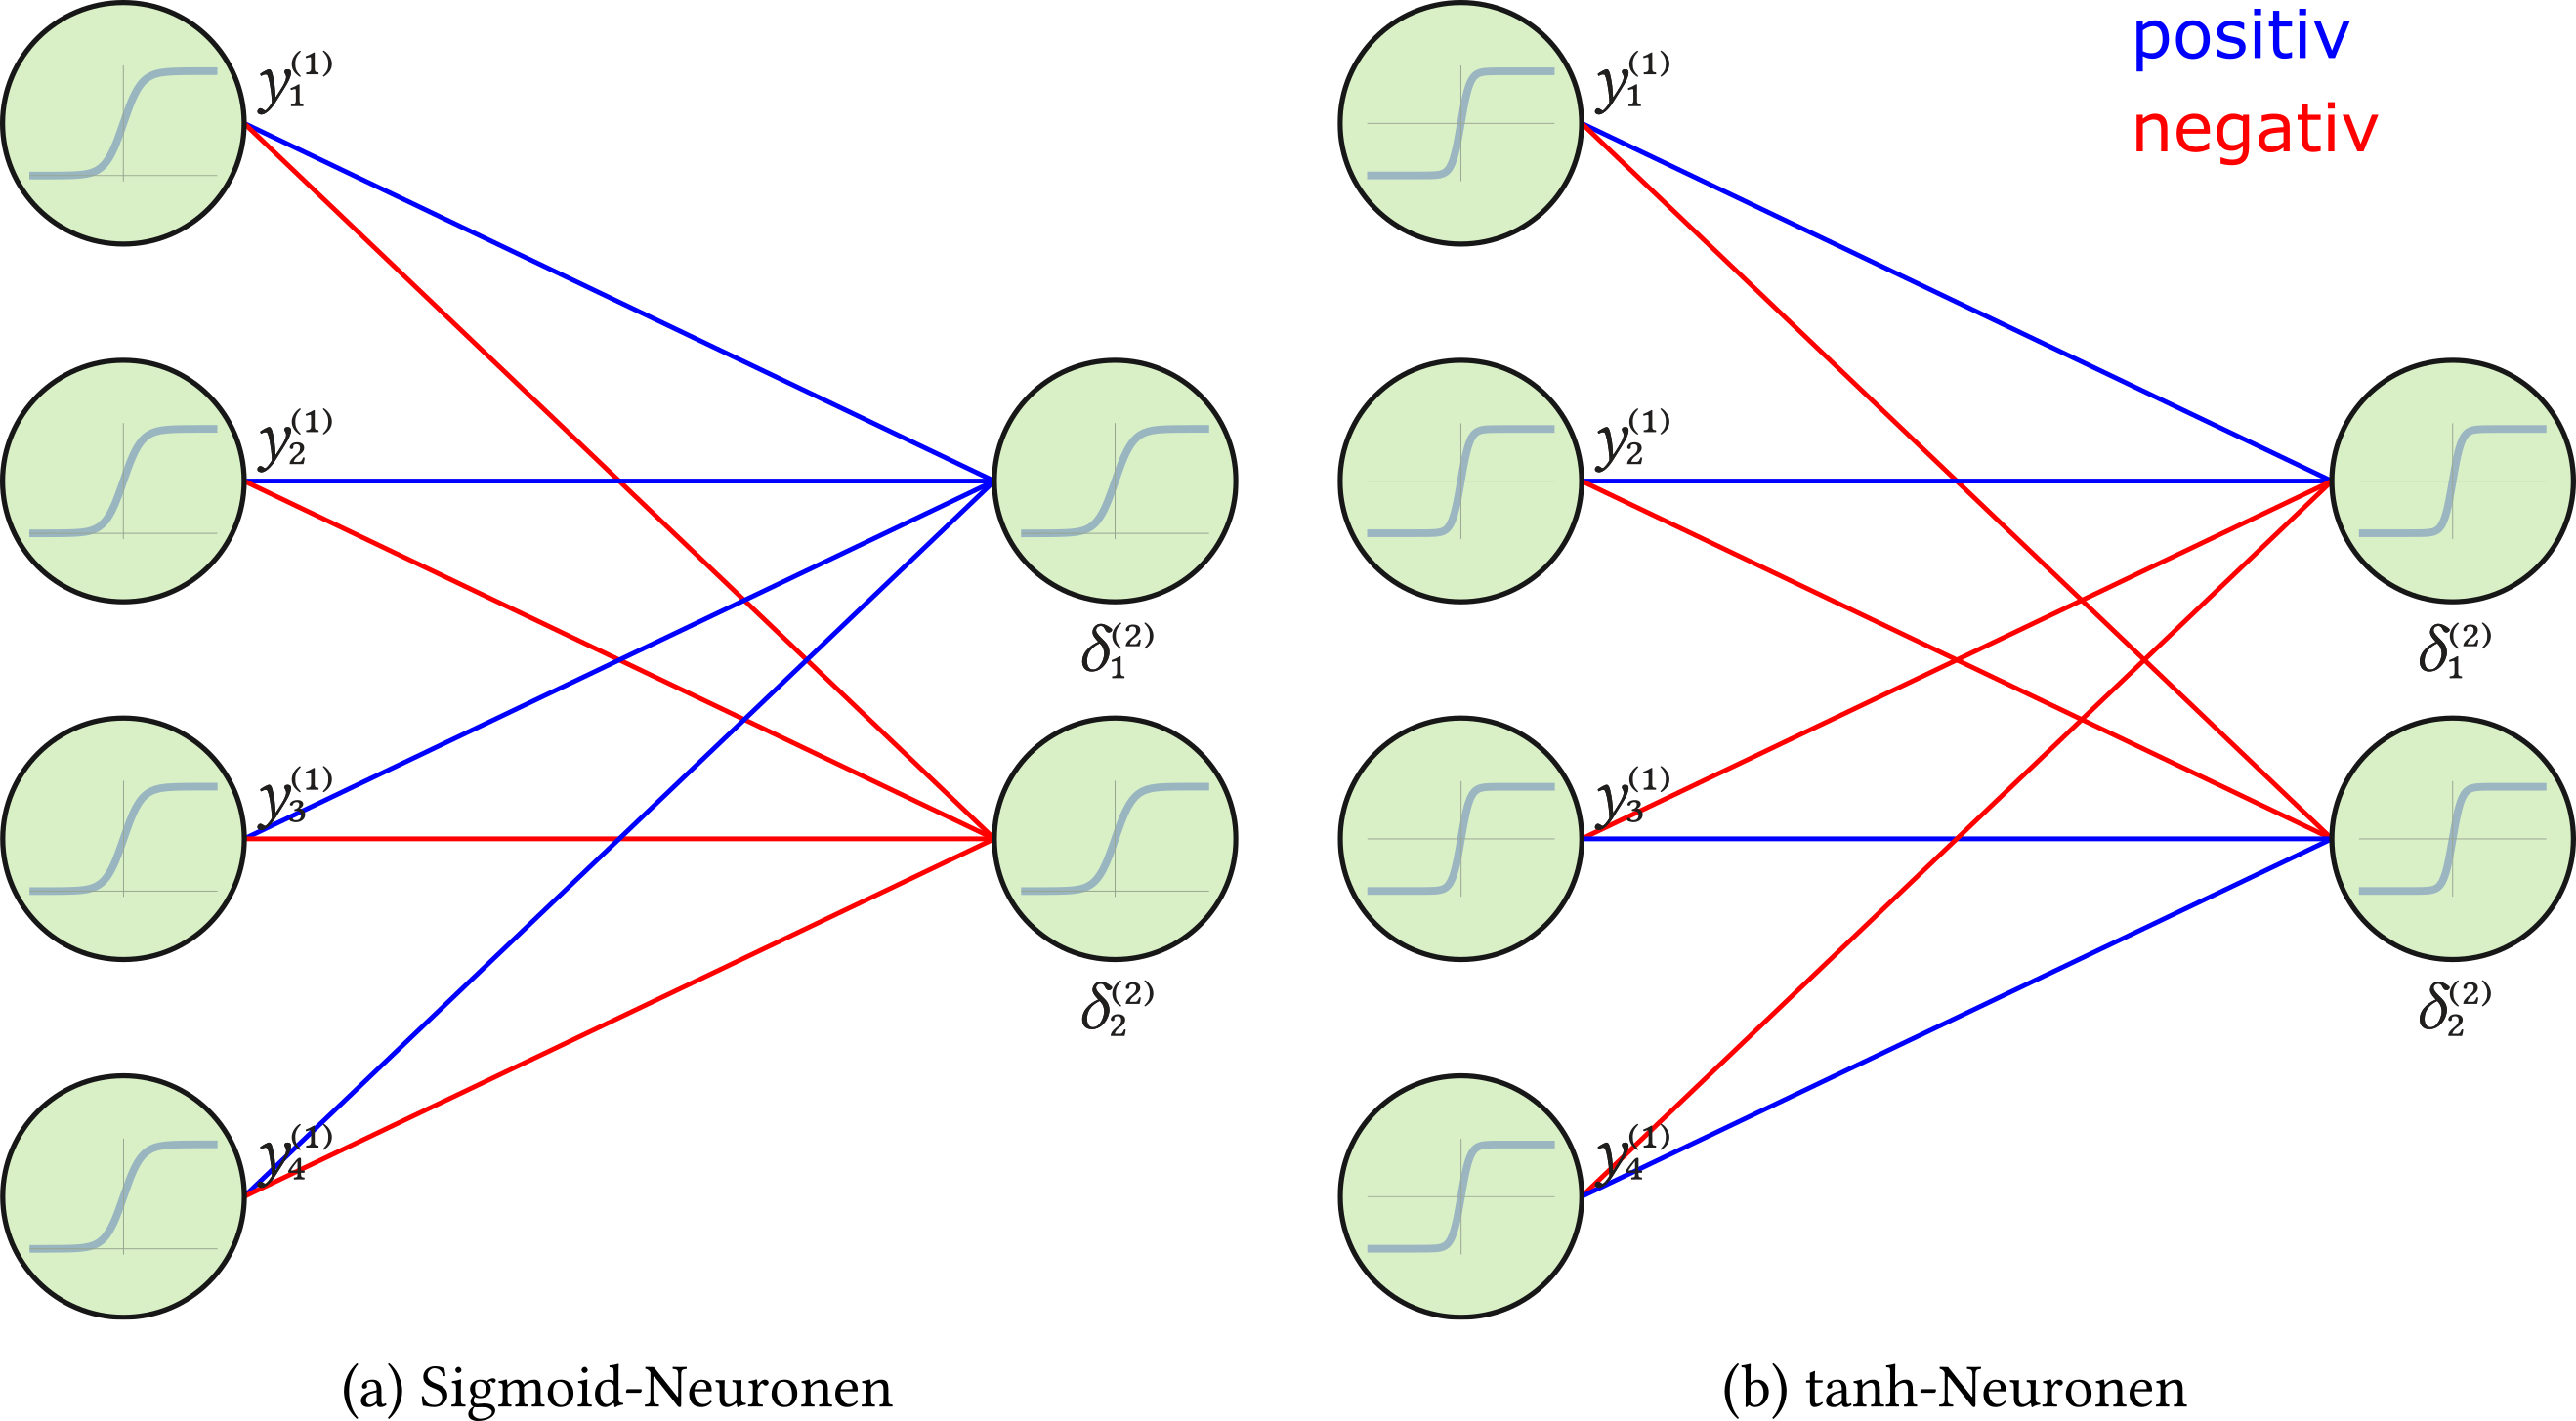
\includegraphics[width = 0.7\textwidth]{1b}\\\end{center}

iii. Die Sigmoid-Funktion ist für alle $x$ positiv, während bei tanh auch negative Werte möglich sind.

\section*{Teilaufgabe 2}

a) Für $x < 0$ gilt: Es wird nicht gelernt.\\
Für $x > 0$ gilt: Je größer $x$, desto schneller wird gelernt.\\
\\
b) Für ReLU(x) wird nur 1 Rechenoperation benötigt, für tanh(x) hingegen 5 Operationen. Man kann also erwarten, dass für ReLU(x) der Lernvorgang schneller ist.\\
\\
c) Für $u_i < 0$ folgt $ReLU(u_i) = 0$ und insbesondere auch für die Ableitung $ReLU'(u_i) = 0$. Somit wird nicht gelernt und die Gewichte verändern sich nicht. Bei $LeakyReLU$ wird dieses Problem umgangen, da die Ableitung immer mindestens $\alpha$ oder 1 ist.

\section*{Teilaufgabe 3}

a) Der Gradient ist bei $ELU_{\alpha}(x)$ um die Stelle $x = 0$ stetig, bei $LeakyReLU$ hat er eine Sprungstelle.\\
\\
b)\\
i. Stark unterschiedliche Verteilungsparameter über die Lernepochen können sehr ungünstig sein, da
\begin{itemize}
	\item die Werte der Gewichte sehr stark schwanken
	\item der Input für die $l + 1$ Schicht stark verschieden ist
\end{itemize}
Somit ist das Lernen sehr ungleichmäßig.\\
\\
ii. Für diesen Fall gilt für die Werte $u <0$:
\begin{itemize}
	\item die Werte verkleinern sich, wodurch sich der Mittelwert $\mu$ näher zur 0 bewegt
	\item je größer der Wert betragsmäßig ist, desto stärker ist die Verkleinerung, wodurch die Standardabweichung $\sigma$ kleiner wird
\end{itemize}

\noindent iii. In diesem Fall werden die Werte für $u \geq 0$ mit $\lambda$ multipliziert und dadurch breiter gestreut.

\section*{Teilaufgabe 4}

a) Die notwendigen Epochen belaufen sich auf:
\begin{itemize}
	\item sig: 2197
	\item tanh: 500
	\item ReLU: 136
\end{itemize}
\begin{center}
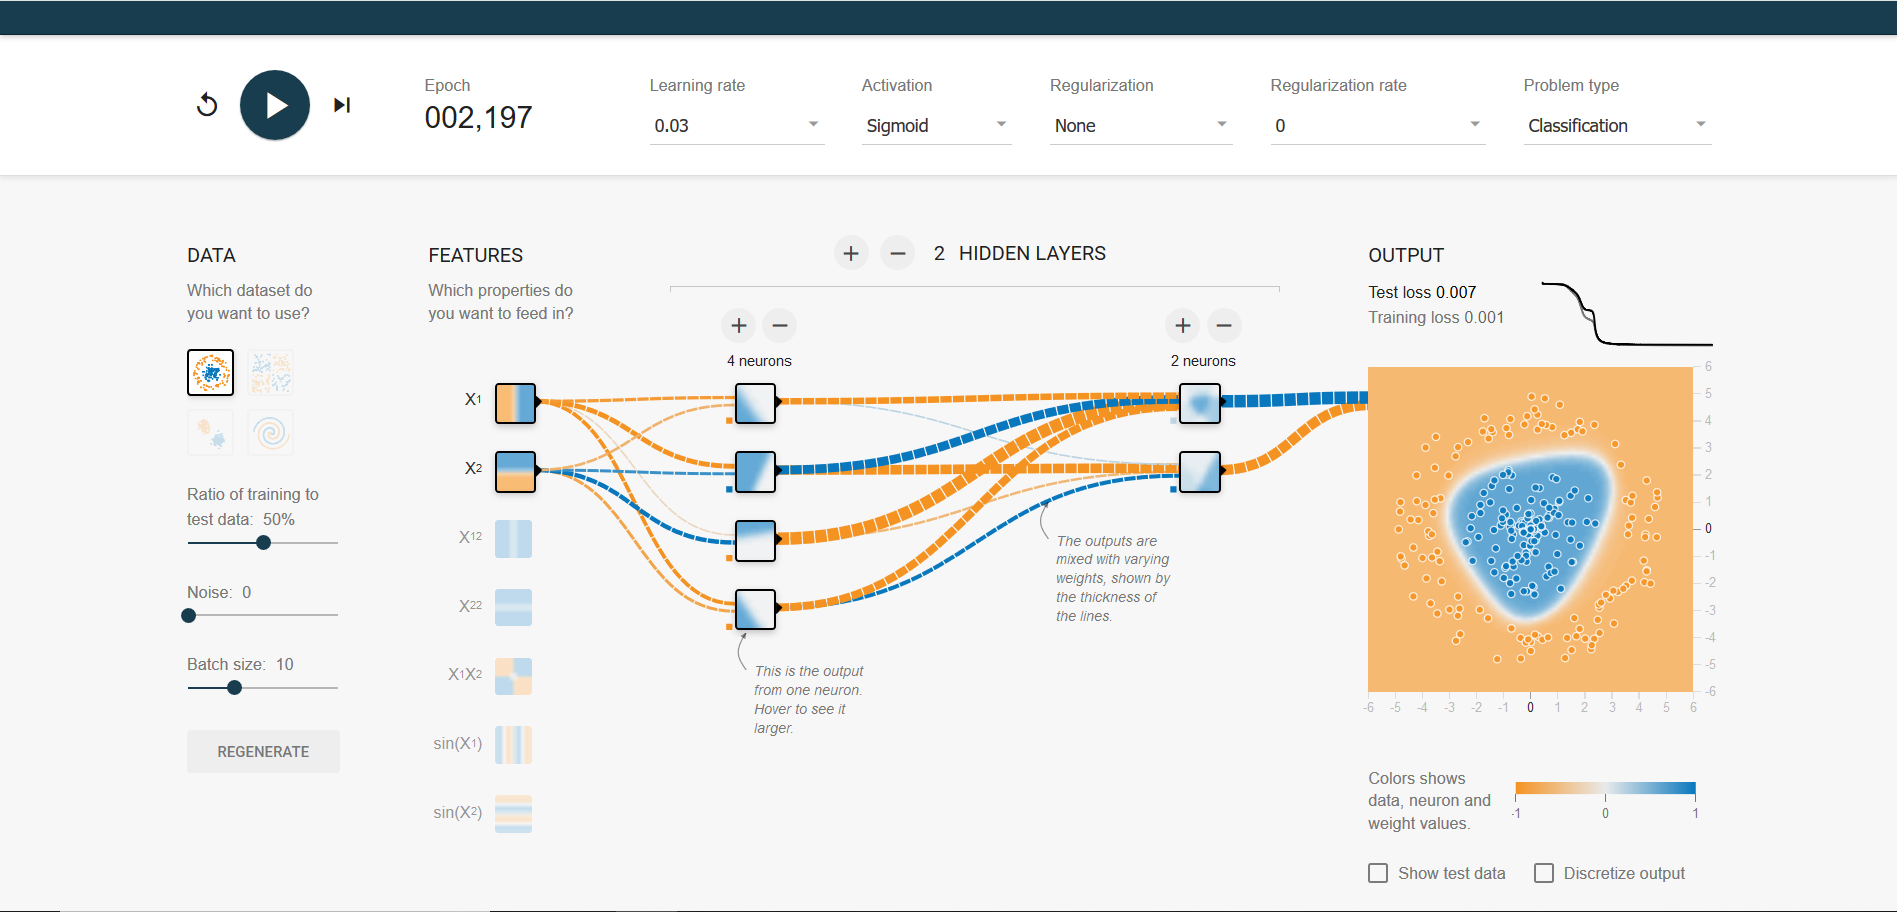
\includegraphics[width = 0.7\textwidth]{sigmoid}\\
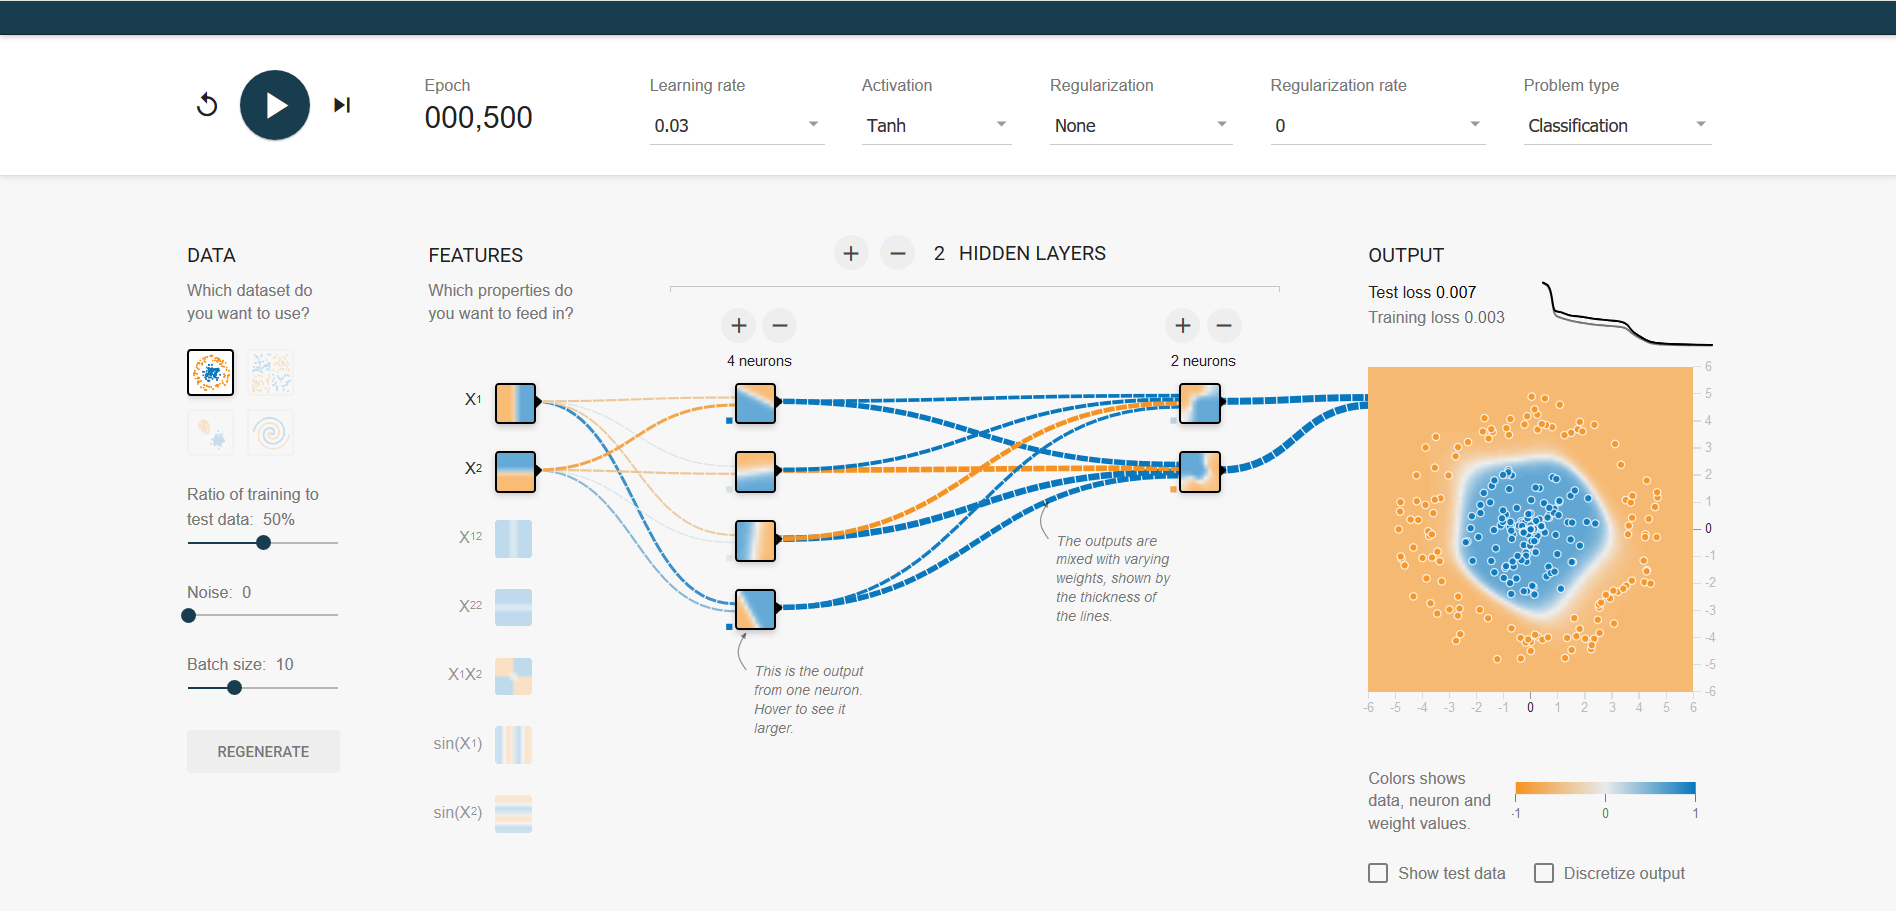
\includegraphics[width = 0.7\textwidth]{tanh}\\
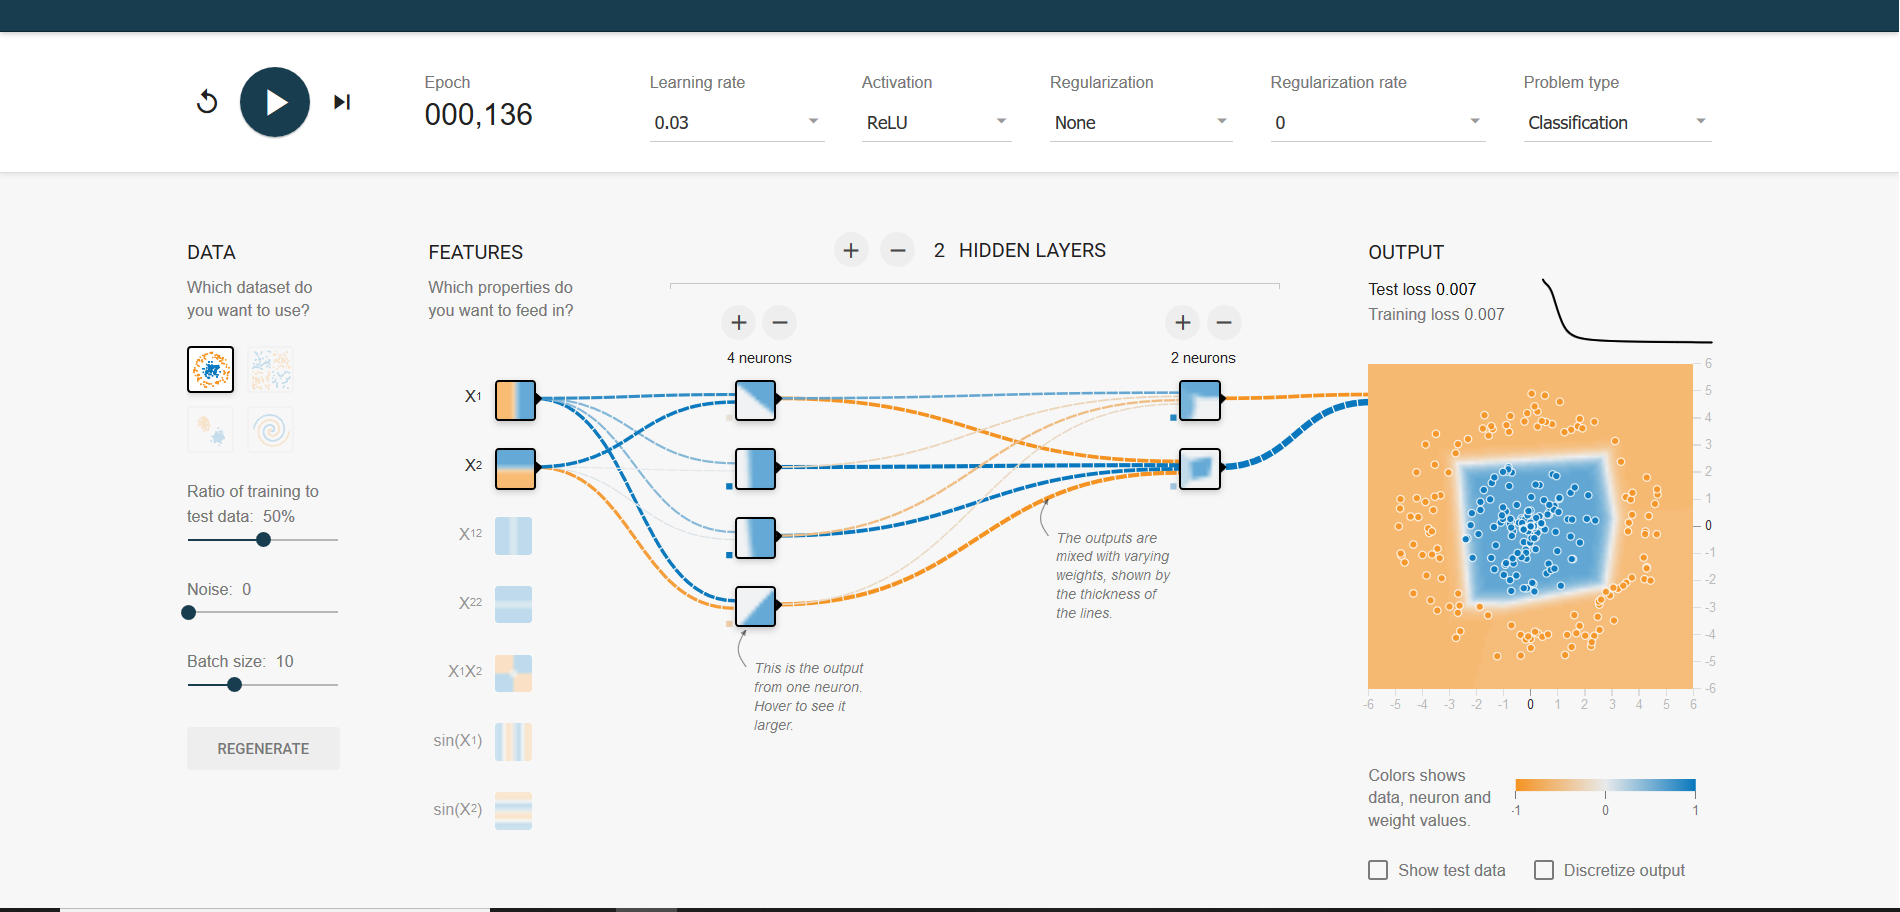
\includegraphics[width = 0.7\textwidth]{relu}\\
\end{center}

b) Für eine Lernrate von $\eta = 10$ wird der Effekt der \textit{dying ReLUs} provoziert.

\section*{Teilaufgabe 5}
a)\\
i. Man stellt in diesem Bereich fest, dass die Aktivitäten von der ersten bis zur letzten Schicht gegen 0 konvergieren, sowie dass die Gradienten in die andere Richtung, also von der letzten zur ersten Schicht ebenfalls gegen 0 konvergieren, für alle Funktionen.\\
\\
ii. Wir betrachten die Aktivitäten. Nimmt man die Absolutwerte der beiden Funktionen, so stellen sich nach wenigen Schichten von der ersten zur letzten gehend betrachtet fast dieselben Werte ein. Nur die Vorzeichen sind invertiert: $ReLU$ ist negativ behaftet, während $ELU$ positiv behaftet ist.\\
\\
iii. Weil der $tanh$ schneller konvergiert.\\
\\
iv. In diesem Beispiel wird mit der $SELU$ Funktion am meisten gelernt.\\
\\
\\
b)\\
$tanh$: Beim $tanh$ konzentrieren sich die Aktivitäten im Bereich von [-0.5, 0.5] der activation und nehmen mit den Schichten beschränkt wachsend zu.\\
\\
$ReLU$: Bei der $ReLU$-Funktion konzentrieren sich die Netzwerk-Aktivitäten auf einen kleinen Bereich um die 0 der Aktivierungen. Bereits bei niedrigen Schichten haben wir hohe Aktivitäten und diese konvergiert recht schnell gegen das Maximum.\\
\\
$ELU$: Bei der $ELU$-Funktion haben wir eine ähnliche Konzentration wie beim $tanh$, nur dass die Aktivitäten mit zunehmender Schicht annähernd linear zunehmen.\\
\\
$SELU$: Bei der $SELU$-Funktion nimmt die Netzwerk-Aktivität mit zunehmender Schicht schnell ab. Für die Aktivierung ist bei -0.5 ein lokales Minimum. Die Funktion ist symmetrisch und hat bei -1 beziehungsweise 0 für Aktivierungen jeweils lokale Maxima.


\end{document}